% ----------------------------------------------------------------------------
% INLETS E OUTLETS
% ----------------------------------------------------------------------------

\chapter{Inlets e outlets}
Os objetos que criamos até agora são inúteis. Não servem para nada. Para serem
mais úteis precisamos permitir que os mesmos se comuniquem com outros objetos
do Pure Data. Isto é feito por meio de Inlets e outlets. Temos dois tipos de
inlets: passivos e ativos. 

\section{Inlets passivos}
Inlets passivos são inlets cuja entrada é associada a um atributo do objeto.
São chamados de passivos pois a alteração do seu valor não irá iniciar a
execução de uma função. Já os inlets ativos são associados a funções e permitem
um pouco mais de ação quando um valor é atribuído.

\begin{lstlisting}
static t_class *example4_class;

typedef struct _example4 {
    t_object x_obj;
    t_float my_float;// Creates a my_float variable into the structure
} t_example4;


// Constructos of the class
void * example4_new(t_symbol * arg1, t_floatarg arg2) {
    t_example4 *x = (t_example4 *) pd_new(example4_class);
    post("First arg: %s", arg1->s_name);
    post("Second arg: %f", arg2);

    floatinlet_new(&x->x_obj, &x->my_float); //create a passive inlet which value will be stored into my_float variable

    return (void *) x;
}
\end{lstlisting}

O inlet passivo depende que a variável que irá armazenar o valor seja do mesmo
tipo que a função usada para a criação do inlet (Veja o exemplo04). Os tipos de
inlets passivos são:

\begin{itemize}
\item floatinlet\_new(t\_object *owner, t\_float *fp)
\item symbolinlet\_new(t\_object *owner, t\_symbol **sp)
\item pointerinlet\_new(t\_object *owner, t\_gpointer *gp)
\end{itemize}

\begin{figure}[h!]
	\centering
	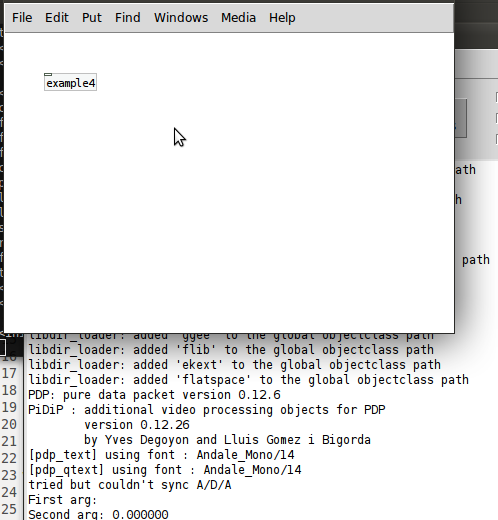
\includegraphics[width=0.7\textwidth]{example4}
	\caption{Inlets passivos}
\end{figure}

\section{Inlets ativo}
Um inlet ativo associa ao inlet uma função. Assim como o inlet passivo, a
criação de um inlet ativo permite definir o tipo do dado que o inlet irá
receber.(Veja o exemplo05).

\begin{lstlisting}
// The method will always receive the class as argument
void example5_bang(t_example5 *x) { 
    post("BANGED!");
    post("My_float value: %f",x->my_float);
}

void example5_anything(t_example5 *x, t_symbol *s, int argc, t_atom *argv){
	post("ANYTHING!");
}

void example5_setup(void) {
    example5_class = class_new(gensym("example5"),
            (t_newmethod) example5_new, // Constructor
            0, 
            sizeof (t_example5),
	    CLASS_DEFAULT,
            0); // LAST argument is ALWAYS zero
    class_addbang(example5_class, example5_bang);
    class_addanything(example5_class, example5_anything);
}
\end{lstlisting}

Este é o resultado:

\begin{figure}[h!]
	\centering
	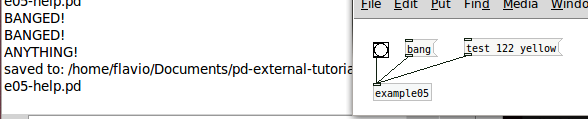
\includegraphics[width=0.7\textwidth]{example5}
	\caption{Inlets.}
\end{figure}

Os tipos definidos na criação de inlets dependem da função que irá receber o
conteúdo deste inlet possuir a assinatura correta. São elas:

\begin{table}[ht]
\centering
\begin{tabular}{ll}
\hline
\hline
void class\_addbang(t\_class *c, t\_method fn); 	& void my\_bang\_method(t\_mydata *x); \\
void class\_addfloat(t\_class *c, t\_method fn);	& void my\_float\_method(t\_mydata *x, t\_floatarg f); \\
void class\_addsymbol(t\_class *c, t\_method fn);	& void my\_symbol\_method(t\_mydata *x,t\_symbol *s); \\
void class\_addpointer(t\_class *c, t\_method fn);	& void my\_pointer\_method(t\_mydata *x, t\_gpointer *pt); \\
void class\_addlist(t\_class *c, t\_method fn);		& void my\_list\_method(t\_mydata *x, t\_symbol *s, int argc, t\_atom *argv); \\
void class\_addanything(t\_class *c, t\_method fn);	& void my\_any\_method(t\_mydata *x, t\_symbol *s, int argc, t\_atom *argv); \\
\hline
\hline
\end{tabular}
\end{table}

\section{Um inlet com várias mensagens}

Um inlet pode ainda receber vários tipos de mensagens diferentes e associar
métodos diferentes para tratar cada tipo de mensagem. Isto é feito com a função
add\_method.  (Veja o exemplo08).

\begin{lstlisting}
// Constructos of the class
void * example8_new(void) {
    t_example8 *x = (t_example8 *) pd_new(example8_class);

    // creating inlets to the messages "alfa"
    inlet_new(&x->x_obj, &x->x_obj.ob_pd, gensym("float"), gensym("alfa"));

    return (void *) x;
}

void example8_start(t_example8 *x){
    post("START / BANG");
}

void example8_open(t_example8 *x, t_symbol *s){
    post("open %s",s->s_name);
}


void example8_alfa(t_example8 *x, t_floatarg f){
	post("ALFA VALUE %f",f);
}

void example8_setup(void) {
    example8_class = class_new(gensym("example8"),
            (t_newmethod) example8_new, // Constructor
            (t_method) example8_destroy, // Destructor
            sizeof (t_example8),
	    CLASS_DEFAULT,
            0); // LAST argument is ALWAYS zero

    // All these messages will be received by the first left inlet
    class_addmethod(example8_class, (t_method) example8_start, 
	gensym("start"), 0); // two messages, the same function
    class_addmethod(example8_class, (t_method) example8_start, 
	gensym("bang"),  0); // may be "start" or "bang" messages
    class_addmethod(example8_class, (t_method) example8_open,  
	gensym("open"),  A_DEFSYMBOL,0);

    // These messages will be associated with inlet 2
    class_addmethod(example8_class, (t_method) example8_alfa,  
	gensym("alfa"), A_DEFFLOAT,0); 

}
\end{lstlisting}

Desta forma não precisamos tratar a mensagem que o inlet recebe mas definí-las
de antemão e criar funções que mapeiem a mensagem recebida.

\begin{figure}[h!]
	\centering
	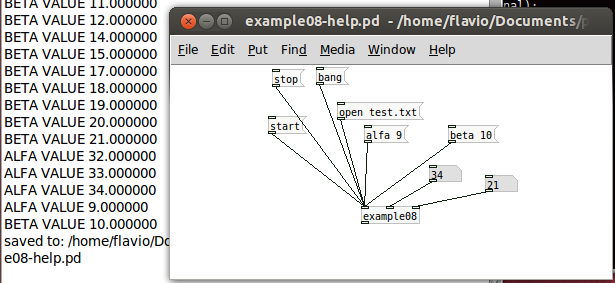
\includegraphics[width=0.7\textwidth]{example8}
	\caption{Mais inlets.}
\end{figure}


Note que este código possui duas abordagens para esta estrutura de inlets. Uma
é associar o tipo da mensagem e o parâmetro a um método e outra é criar um
inlet "genérico" que vai associar a mensagem a um novo inlet. Isto é feito pela
função inlet\_new.

\begin{lstlisting}
t_inlet *inlet_new(t_object *owner, t_pd *dest,
      t_symbol *s1, t_symbol *s2);
\end{lstlisting}

\section{Oulets}

Depois de termos tratados as formas de entrada de dados para o inlet do PD,
chegou a hora de tratarmos as saídas. Isto é feito por meio de outlets. (Veja o
exemplo06).

\begin{lstlisting}

typedef struct _example6 {
    t_object x_obj;
    t_outlet *my_outlet; // Defines an outlet
} t_example6;

// The BANG method, first inlet

void example6_bang(t_example6 *x) {
    post("BANGED!");
    outlet_bang(x->my_outlet); // Bang my outlet
}

// Constructos of the class
void * example6_new(t_symbol * arg1, t_floatarg arg2) {
    t_example6 *x = (t_example6 *) pd_new(example6_class);

    x->my_outlet = outlet_new(&x->x_obj, gensym("bang"));

    return (void *) x;
}

void example6_setup(void) {
    example6_class = class_new(gensym("example6"),
            (t_newmethod) example6_new, // Constructor
            0, 
            sizeof (t_example6),
	    CLASS_DEFAULT,
            A_DEFFLOAT, // First Constructor parameter
            A_DEFSYMBOL, // Second Consctructo parameter
            0); // LAST argument is ALWAYS zero
    class_addbang(example6_class, example6_bang);
}
\end{lstlisting}

Um outlet deve ser definido na estrutura do objeto e instanciado pela função
outlet\_new. Isto permite também definirmos o tipo de dado que ele terá. No
caso deste exemplo, o outlet possui um bang e disparará o bang toda vez que
receber um bang.

\begin{figure}[h!]
	\centering
	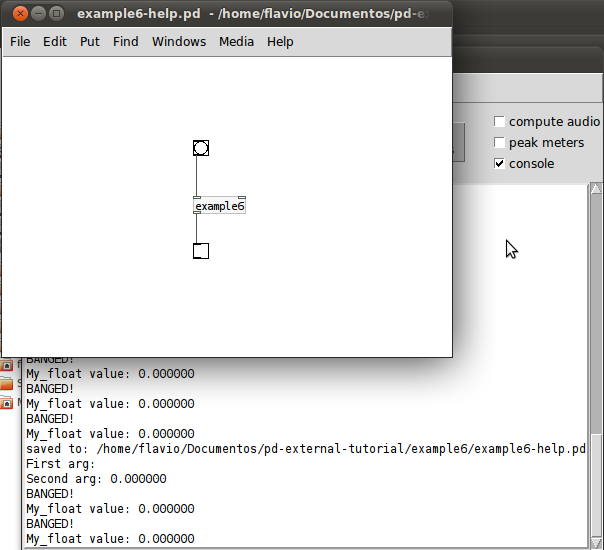
\includegraphics[width=0.7\textwidth]{example6}
	\caption{Um external bem útil que recebe um bang e envia um bang.}
\end{figure}

\todo{Tem um tipo de inlet/outlet que utiliza um sistema de proxy para que os
mesmos possam ser definidos on the fly. Nunca usei mas acho que seria legal abordar.
 Ele baseia-se em definir um método em outro objeto (o proxy) e associar
este novo inlet ao proxy. Assim podemos instanciar vários proxys e tratar vários
inlets passivos, por exemplo.}
